% Created 2025-04-29 Tue 19:39
% Intended LaTeX compiler: pdflatex
\documentclass[11pt]{article}
\usepackage[utf8]{inputenc}
\usepackage[T1]{fontenc}
\usepackage{graphicx}
\usepackage{longtable}
\usepackage{wrapfig}
\usepackage{rotating}
\usepackage[normalem]{ulem}
\usepackage{amsmath}
\usepackage{amssymb}
\usepackage{capt-of}
\usepackage{hyperref}
\usepackage{minted}
\usepackage{graphicx}
\graphicspath{ {./images/} }
\author{Hankertrix}
\date{\today}
\title{Angular Momentum Notes}
\hypersetup{
 pdfauthor={Hankertrix},
 pdftitle={Angular Momentum Notes},
 pdfkeywords={},
 pdfsubject={},
 pdfcreator={Emacs 30.1 (Org mode 9.7.11)}, 
 pdflang={English}}
\begin{document}

\maketitle
\setcounter{tocdepth}{2}
\tableofcontents \clearpage\section{Definitions}
\label{sec:org69873b1}

\subsection{Torque (\(\tau\))}
\label{sec:org372c29e}
Torque is a measure of the force that can cause an object to rotate about a point, in this case, point \(O\). It is also called the moment of a force. It is given by:
\[\tau = \vec{r} \times \vec{F}\]

Where \(\vec{r}\) is the perpendicular distance of the object from a point \(O\), and \(\vec{F}\) is the force acting on the object.
\subsection{Power (\(P\))}
\label{sec:org444e8f8}
The power of a rotating object with \textbf{constant torque} is given by:
\[P = \tau \omega\]

\newpage
\subsection{Right-hand rule}
\label{sec:orgbc52c34}
When the fingers of your right hand are curled in the direction of rotation, your right thumb points in the direction of \(\vec{\omega}\). If the rotation axis is also an axis of symmetry, this is also the direction of \(\vec{L}\).

\[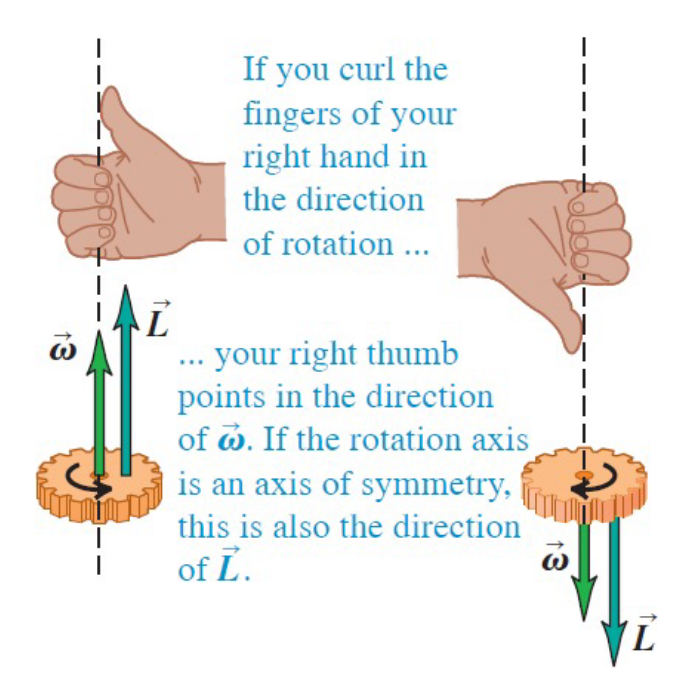
\includegraphics[width = \textwidth]{right-hand-rule}\]

\newpage
\subsection{Conservation of angular momentum}
\label{sec:org2fcfb08}
When the net external torque acting on a system is zero, the total angular momentum of the system is constant.


Essentially:
\[\frac{dL}{dt} = 0\]
\[L = I \vec{\omega} = \text{constant}\]
\subsection{Precession}
\label{sec:orgd465672}
Precession is the slow movement of the axis of a spinning body around another axis due to a torque, such as gravitational influence acting to change the direction of the first axis. It is seen in the circle slowly traced out by the pole of a spinning gyroscope.
\section{Formulas}
\label{sec:org6a5db6c}

\subsection{Angular momentum (\(L\))}
\label{sec:org268d8e3}
The angular momentum of a point object rotating around a point \(O\) is given by:
\[\vec{L} = \vec{r} \times \vec{p}\]
\[\vec{L} = \vec{r} \times m \vec{v}\]
\[\vec{L} = r \sin \theta \cdot m \vec{v}\]

Where \(\vec{r}\) is the distance of the object from the point \(O\), \(\vec{p}\) is the linear momentum of the object and \(\vec{v}\) is the velocity of the object.


The angular momentum (\(L\)) of a rigid body rotating around a symmetry axis is given by:
\[\vec{L} = I \vec{\omega}\]

\begin{itemize}
\item \(I\) is the moment of inertia of rigid body about the symmetry axis
\item \(\vec{\omega}\) is the angular velocity vector of the rigid body
\end{itemize}

If the axis is \textbf{not} an axis of symmetry, or \textbf{not} parallel to the angular velocity, the above relation holds, but the moment of inertia is written as a 3 by 3 matrix.

\newpage
\subsection{Rate of change of total angular momentum}
\label{sec:org3b5d553}
For any system of particles, the rate of change of the total angular momentum equals the sum of the torques of all forces acting on all the particles:

\[\sum \vec{\tau} = \frac{d \vec{L}}{dt}\]
\[\sum \vec{\tau} = I \alpha\]

This is only valid when the net external torque, and the angular moment \(L\), are calculated with respect to either:
\begin{enumerate}
\item The origin of an inertial reference frame.
\item The \textbf{centre of mass} of a system of particles or rigid body.
\end{enumerate}
\section{Flywheel}
\label{sec:org5fe6686}

\subsection{Non-rotating flywheel}
\label{sec:org16e3367}
When the flywheel is not rotating, its weight creates a torque around the pivot, causing is to fall along a circular path until its axis rests on the table surface.


In falling, the flywheel rotates about the pivot and thus acquires an angular momentum \(\vec{L}\). The direction of \(\vec{L}\) stays constant.
\subsection{Rotating flywheel}
\label{sec:orgda2ba0e}
When the flywheel is rotating, the system starts with an angular momentum \(\vec{L_i}\) parallel to the flywheel's axis of rotation.


Now when the flywheel falls, the effect of the torque due to the weight is to cause the angular momentum to precess around the pivot. The gyroscope circles around is pivot \textbf{without falling}.

\newpage
\section{Derivation of the precession rate of gyroscopes}
\label{sec:org1b71bc8}
Changes in angular momentum as a result of external torque due to weight is:
\[d \vec{L} = \vec{\tau}_{ext} \, dt\]
\[dL = L \sin \theta \, d \phi\]

The angular velocity of precession is:
\begin{align*}
\Omega &= \frac{d \phi}{dt} \\
&= \frac{1}{L \sin \theta} \frac{dL}{dt} \\
&= \frac{\tau_{ext}}{L \sin \theta} \\
&= \frac{M gr \sin \theta}{L \sin \theta} \\
&= \frac{Mgr}{L} \\
&= \frac{Mgr}{(kMR_0^2) \omega} \\
&= \frac{gr}{kR_0^2 \omega}
\end{align*}

\begin{itemize}
\item \(k\) is the dimensionless pre-factor of the moment of inertia
\item \(R_0\) is the radius of the flywheel
\end{itemize}

The angular velocity of precession in general is:
\[\Omega = \frac{\tau_{ext}}{L \sin \theta}\]
\section{Moment of inertia for various objects}
\label{sec:org3066cc0}
\[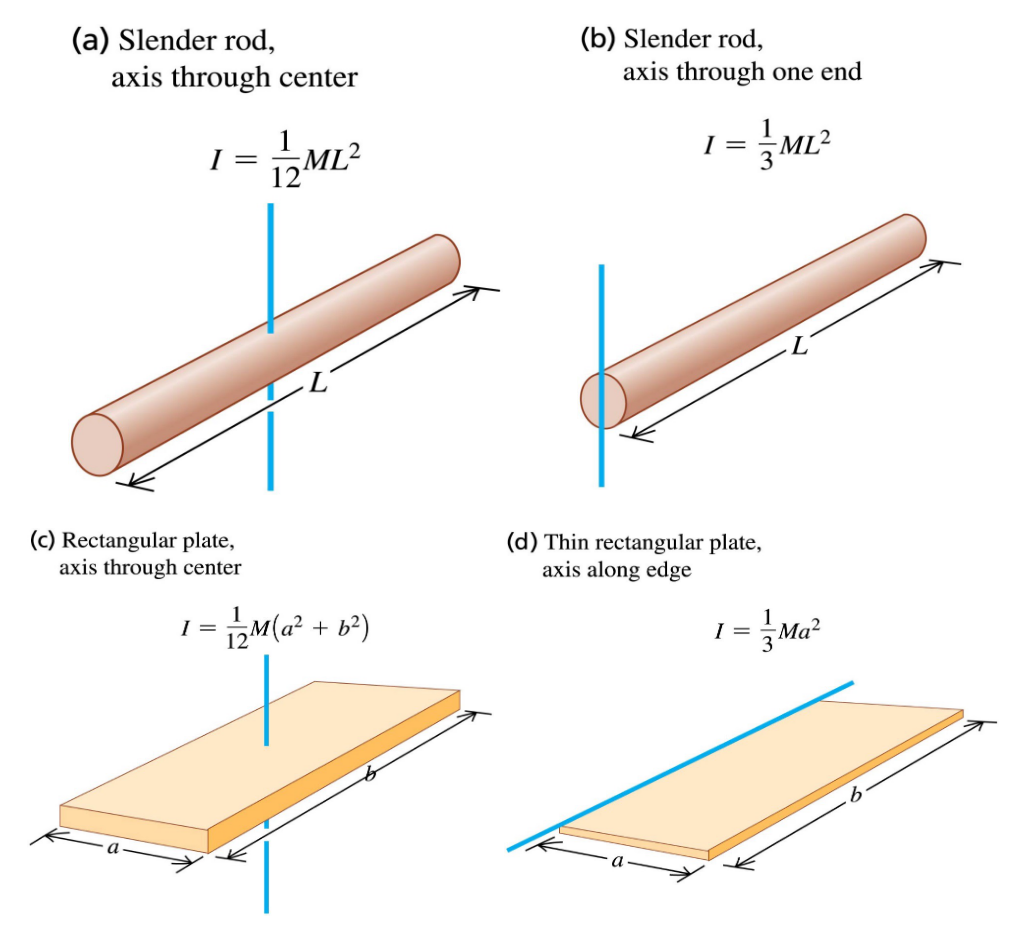
\includegraphics[width = \textwidth]{moments-of-inertia-1}\]
\[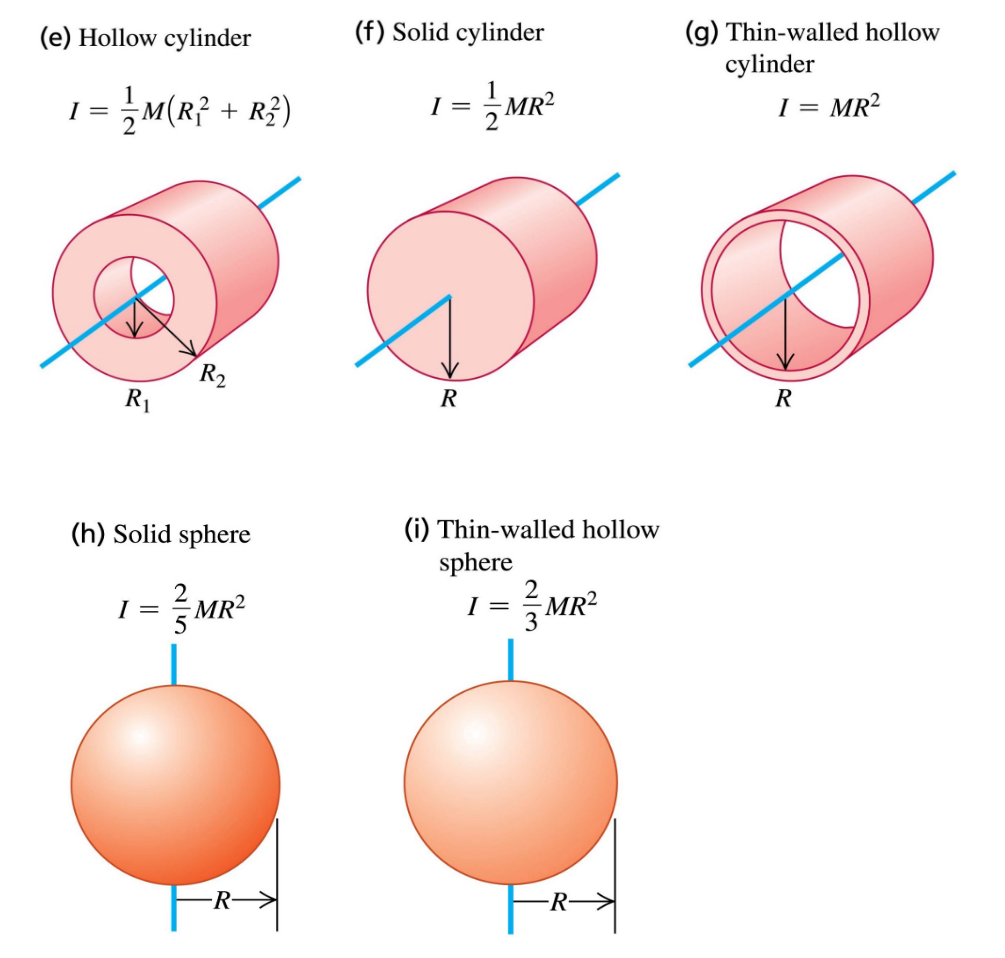
\includegraphics[width = \textwidth]{moments-of-inertia-2}\]
\end{document}
